\documentclass[../main.tex]{subfiles}
\graphicspath{{\subfix{../images/}}}
\begin{document}
\label{Ex:tibetan}
\index{exercises!tibetan}
\index{exercises!statolith}

{I'm presenting here two out of the original five Tibetan Rites. These two are especially interesting in our context, as that they allow the statolith ball to be put in a rotation.}

\vspace{1cm}
\noindent
\begin{tabular}{p{5.4cm} p{6.5cm}}
  \raisebox{-1.4\totalheight}{  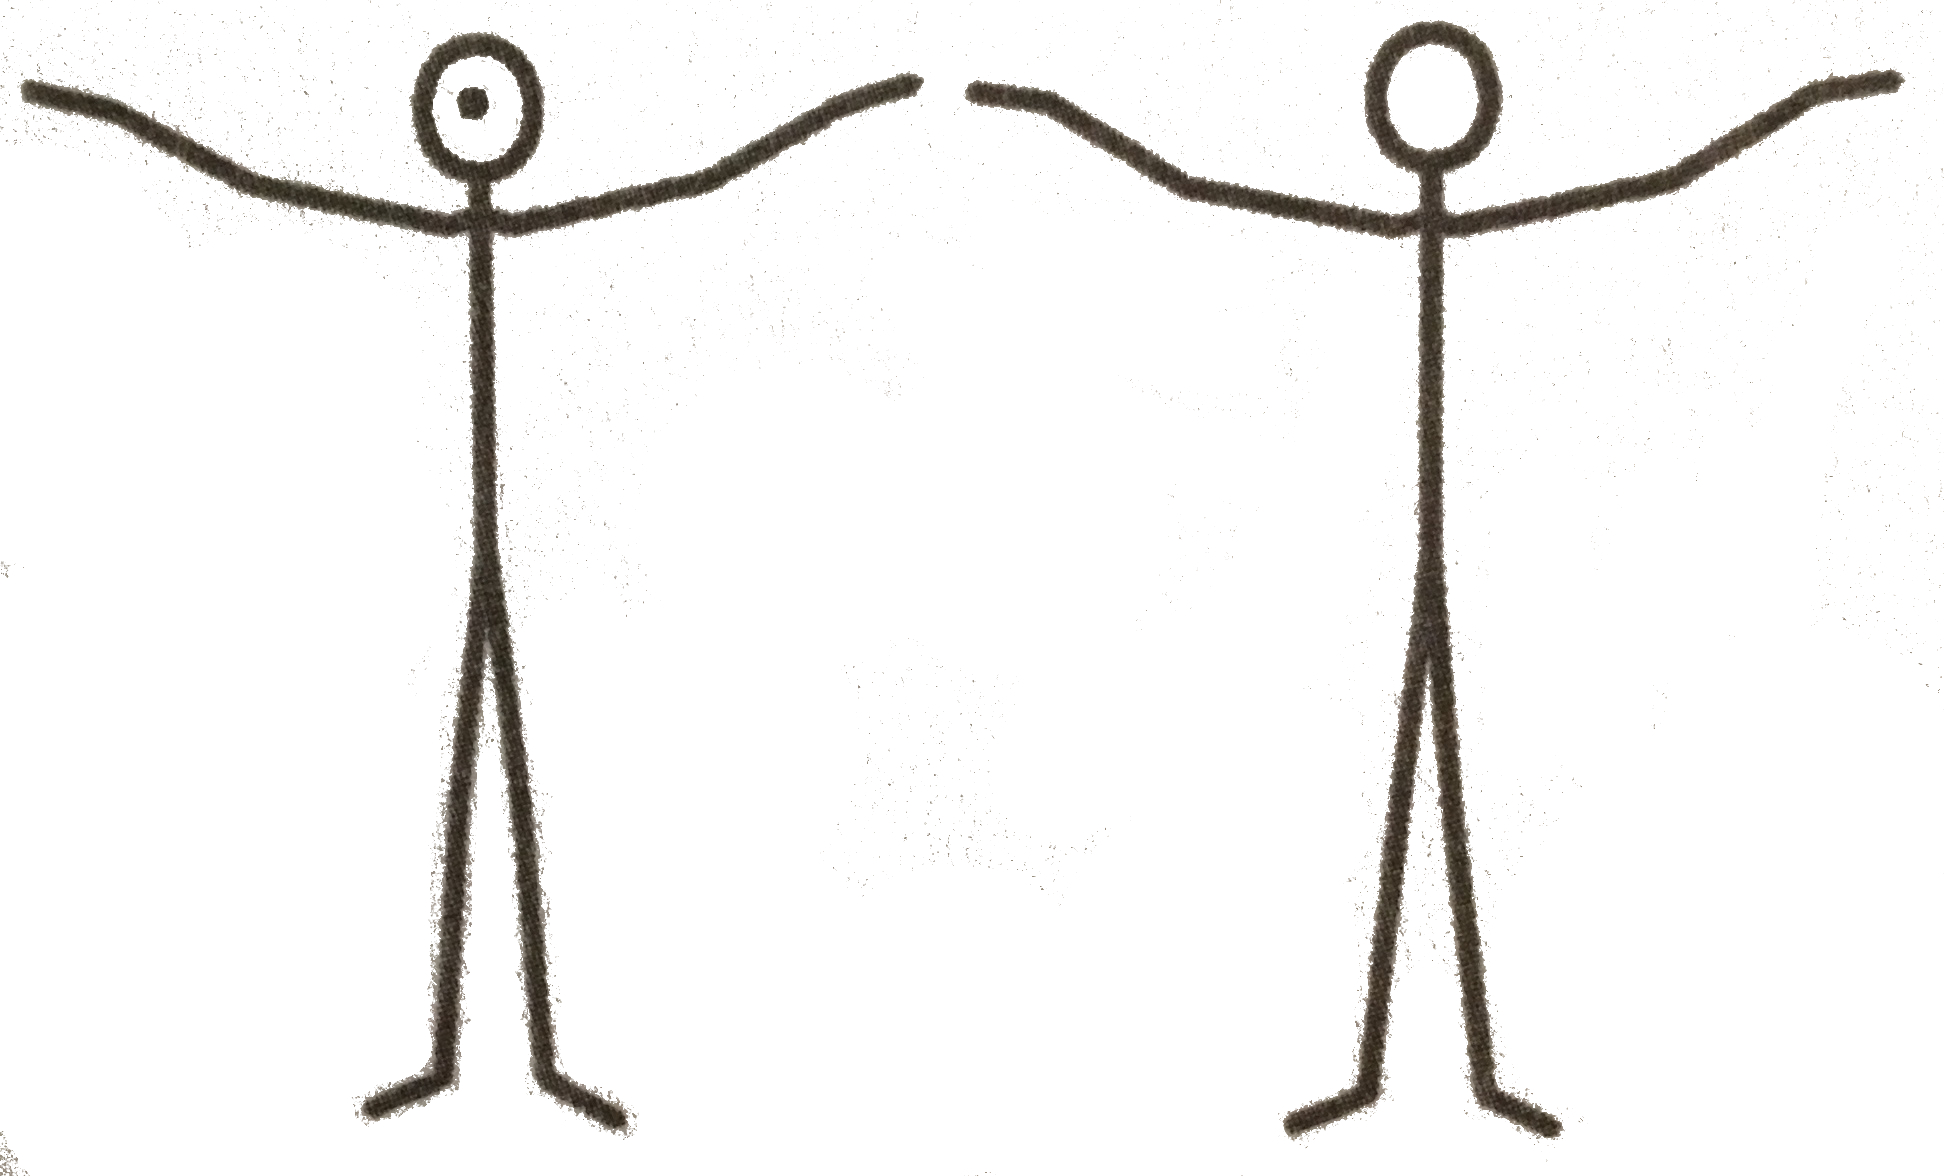
\includegraphics[width=4.3cm]{Tibetan_rotate} }\label{sf:tibetan}
&
\textbf{Tibetan rotation:}


The {arms} are {extended sidewards}, the elbows are slightly flexed, the hands almost shoulder height, the fingers slightly spread. 

{Focus a point} with your eyes. Make little steps and {turn your body} on the spot to the right, the {head stays in place}. 


As soon as you can't hold the point anymore with your head, {swivel your head swiftly} around and focus on a point in the opposite direction. The feet and the body continue to turn.

After a while you can {turn faster}, lift your heels off the floor.


\vspace{2cm}
  \\
  
  \raisebox{-1.4\totalheight}{  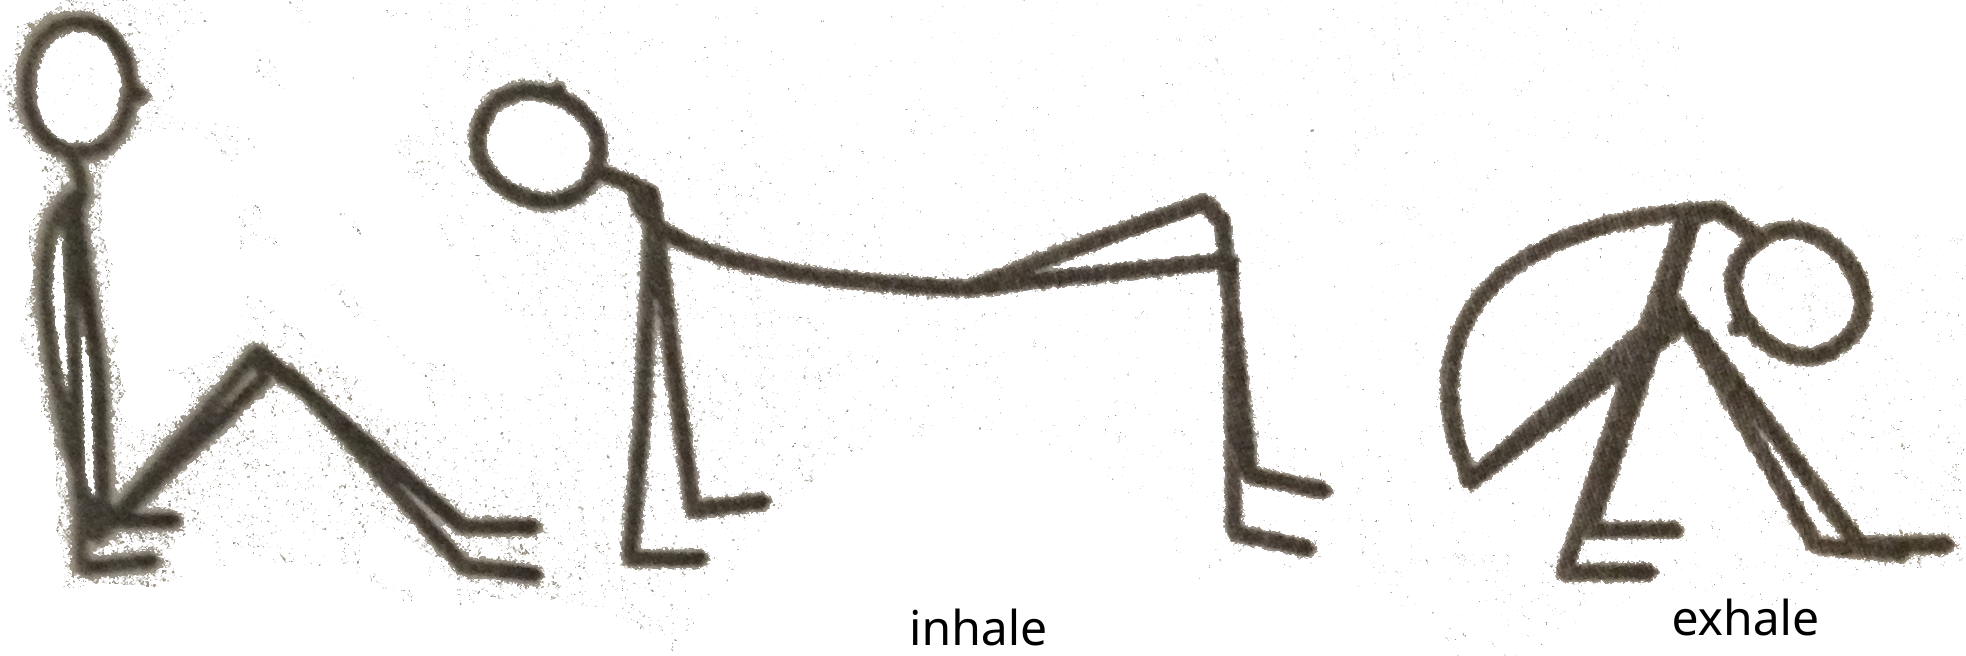
\includegraphics[width=5.4cm]{Tibetan_swing} }
&
\textbf{Tibetan Swing:}

Sit on the floor and put your feet on the ground, the hands are besides your hip.

{Lift your hip} and lead it to the front and up.

{Inhale} while letting your {head roll back} (it's not an own movement, the head just rolls due to the movement of the hip).

Now lead your {hip down and back} and let the {head roll deeply forward}, while exhaling (keep the muscles in the neck relaxed).

Swing with your body forth and back and let your head roll with the movement. After a while you can increase the speed of the swinging.
\end{tabular}
\newpage

\end{document}